\documentclass{standalone}
\usepackage{tikz}
\usetikzlibrary{patterns, positioning}


\begin{document}
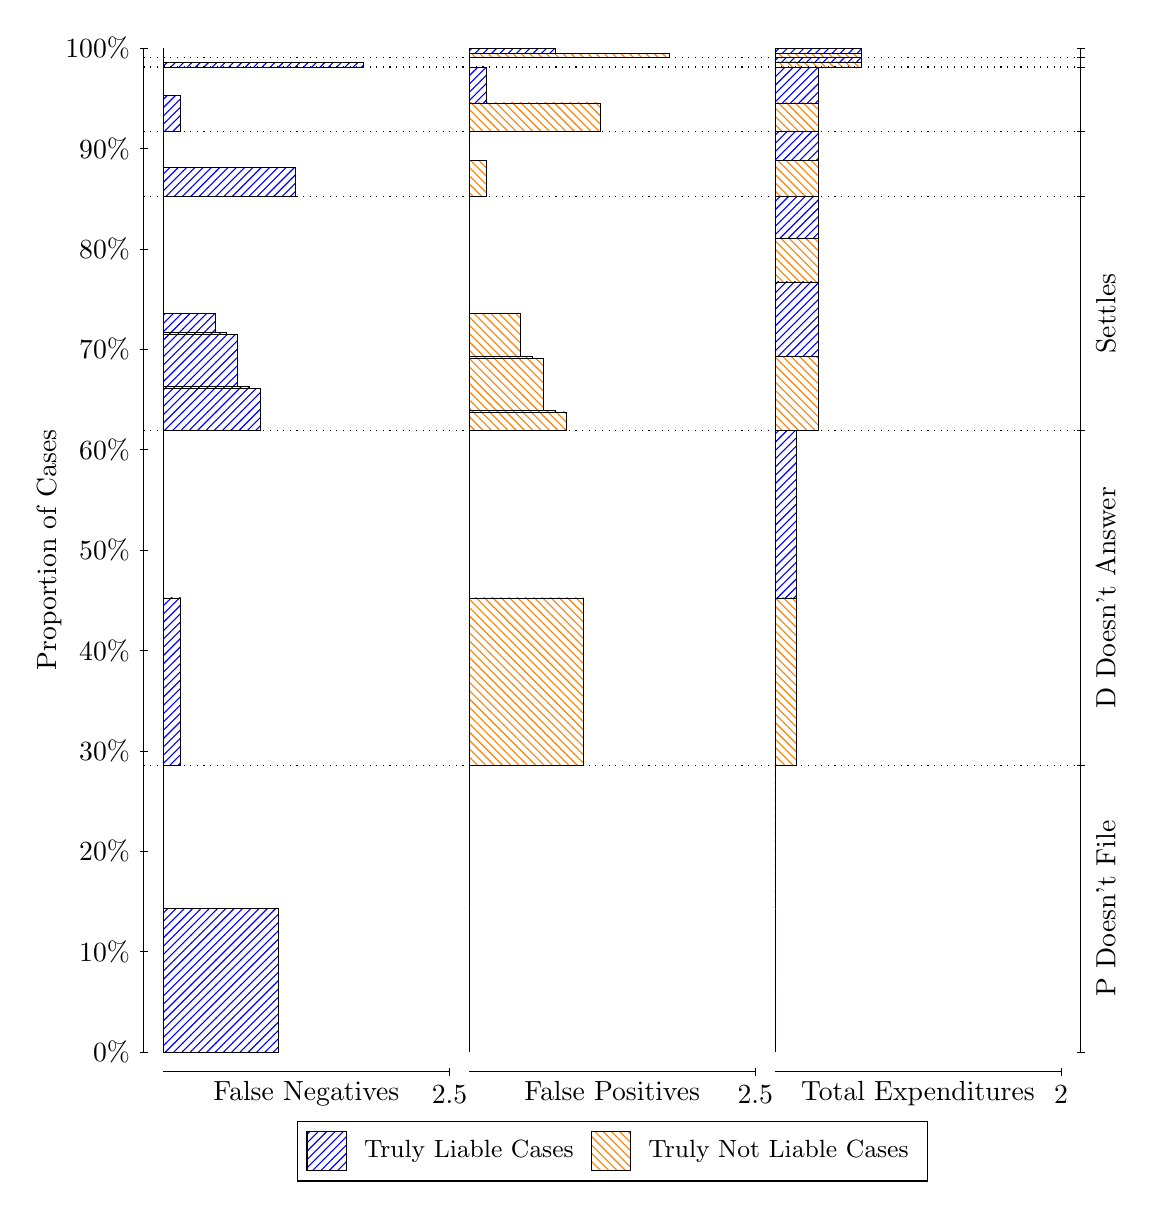
\begin{tikzpicture}
\draw[black, very thin] (1.5,1.75) -- (1.5,14.5);
\node[rotate=90, text=black, anchor=center] at (0.3, 8.125) {Proportion of Cases};
\draw[black, very thin] (1.45,1.75) -- (1.55,1.75);
\node[text=black, anchor=east] at (1.45, 1.75) {0\%};
\draw[black, very thin] (1.45,3.025) -- (1.55,3.025);
\node[text=black, anchor=east] at (1.45, 3.025) {10\%};
\draw[black, very thin] (1.45,4.3) -- (1.55,4.3);
\node[text=black, anchor=east] at (1.45, 4.3) {20\%};
\draw[black, very thin] (1.45,5.575) -- (1.55,5.575);
\node[text=black, anchor=east] at (1.45, 5.575) {30\%};
\draw[black, very thin] (1.45,6.85) -- (1.55,6.85);
\node[text=black, anchor=east] at (1.45, 6.85) {40\%};
\draw[black, very thin] (1.45,8.125) -- (1.55,8.125);
\node[text=black, anchor=east] at (1.45, 8.125) {50\%};
\draw[black, very thin] (1.45,9.4) -- (1.55,9.4);
\node[text=black, anchor=east] at (1.45, 9.4) {60\%};
\draw[black, very thin] (1.45,10.675) -- (1.55,10.675);
\node[text=black, anchor=east] at (1.45, 10.675) {70\%};
\draw[black, very thin] (1.45,11.95) -- (1.55,11.95);
\node[text=black, anchor=east] at (1.45, 11.95) {80\%};
\draw[black, very thin] (1.45,13.225) -- (1.55,13.225);
\node[text=black, anchor=east] at (1.45, 13.225) {90\%};
\draw[black, very thin] (1.45,14.5) -- (1.55,14.5);
\node[text=black, anchor=east] at (1.45, 14.5) {100\%};

\draw[black, very thin] (13.4,1.75) -- (13.4,14.5);
\draw[black, very thin] (13.35,1.75) -- (13.45,1.75);
\node[anchor=west] at (13.35, 1.75) {};
\draw[black, very thin] (13.35,5.3929) -- (13.45,5.3929);
\node[anchor=west] at (13.35, 5.3929) {};
\draw[black, very thin] (13.35,9.6429) -- (13.45,9.6429);
\node[anchor=west] at (13.35, 9.6429) {};
\draw[black, very thin] (13.35,12.618) -- (13.45,12.618);
\node[anchor=west] at (13.35, 12.618) {};
\draw[black, very thin] (13.35,13.438) -- (13.45,13.438);
\node[anchor=west] at (13.35, 13.438) {};
\draw[black, very thin] (13.35,14.259) -- (13.45,14.259);
\node[anchor=west] at (13.35, 14.259) {};
\draw[black, very thin] (13.35,14.38) -- (13.45,14.38);
\node[anchor=west] at (13.35, 14.38) {};
\draw[black, very thin] (13.35,14.5) -- (13.45,14.5);
\node[anchor=west] at (13.35, 14.5) {};

\draw[black, very thin, pattern color=blue, pattern=north east lines] (1.75,1.75) rectangle (3.2033,3.5714);
\draw[black, very thin, pattern color=orange, pattern=north west lines] (1.75,3.5714) rectangle (1.75,5.3929);
\draw[black, very thin, pattern color=blue, pattern=north east lines] (1.75,5.3929) rectangle (1.968,7.5179);
\draw[black, very thin, pattern color=orange, pattern=north west lines] (1.75,7.5179) rectangle (1.75,9.6429);
\draw[black, very thin, pattern color=blue, pattern=north east lines] (1.75,9.6429) rectangle (2.9853,10.182);
\draw[black, very thin, pattern color=blue, pattern=north east lines] (1.75,10.182) rectangle (2.84,10.206);
\draw[black, very thin, pattern color=blue, pattern=north east lines] (1.75,10.206) rectangle (2.6947,10.864);
\draw[black, very thin, pattern color=blue, pattern=north east lines] (1.75,10.864) rectangle (2.5493,10.885);
\draw[black, very thin, pattern color=blue, pattern=north east lines] (1.75,10.885) rectangle (2.404,11.13);
\draw[black, very thin, pattern color=orange, pattern=north west lines] (1.75,11.13) rectangle (1.75,12.618);
\draw[black, very thin, pattern color=blue, pattern=north east lines] (1.75,12.618) rectangle (3.4213,12.981);
\draw[black, very thin, pattern color=orange, pattern=north west lines] (1.75,12.981) rectangle (1.75,13.438);
\draw[black, very thin, pattern color=blue, pattern=north east lines] (1.75,13.438) rectangle (1.968,13.896);
\draw[black, very thin, pattern color=orange, pattern=north west lines] (1.75,13.896) rectangle (1.75,14.259);
\draw[black, very thin, pattern color=blue, pattern=north east lines] (1.75,14.259) rectangle (4.2933,14.315);
\draw[black, very thin, pattern color=orange, pattern=north west lines] (1.75,14.315) rectangle (1.75,14.38);
\draw[black, very thin, pattern color=orange, pattern=north west lines] (1.75,14.38) rectangle (1.75,14.435);
\draw[black, very thin, pattern color=blue, pattern=north east lines] (1.75,14.435) rectangle (1.75,14.5);
\draw[black, very thin, pattern color=orange, pattern=north west lines] (5.6333,1.75) rectangle (5.6333,3.5714);
\draw[black, very thin, pattern color=blue, pattern=north east lines] (5.6333,3.5714) rectangle (5.6333,5.3929);
\draw[black, very thin, pattern color=orange, pattern=north west lines] (5.6333,5.3929) rectangle (7.0867,7.5179);
\draw[black, very thin, pattern color=blue, pattern=north east lines] (5.6333,7.5179) rectangle (5.6333,9.6429);
\draw[black, very thin, pattern color=orange, pattern=north west lines] (5.6333,9.6429) rectangle (6.8687,9.8786);
\draw[black, very thin, pattern color=orange, pattern=north west lines] (5.6333,9.8786) rectangle (6.7233,9.9026);
\draw[black, very thin, pattern color=orange, pattern=north west lines] (5.6333,9.9026) rectangle (6.578,10.561);
\draw[black, very thin, pattern color=orange, pattern=north west lines] (5.6333,10.561) rectangle (6.4327,10.581);
\draw[black, very thin, pattern color=orange, pattern=north west lines] (5.6333,10.581) rectangle (6.2873,11.13);
\draw[black, very thin, pattern color=blue, pattern=north east lines] (5.6333,11.13) rectangle (5.6333,12.618);
\draw[black, very thin, pattern color=orange, pattern=north west lines] (5.6333,12.618) rectangle (5.8513,13.075);
\draw[black, very thin, pattern color=blue, pattern=north east lines] (5.6333,13.075) rectangle (5.6333,13.438);
\draw[black, very thin, pattern color=orange, pattern=north west lines] (5.6333,13.438) rectangle (7.3047,13.802);
\draw[black, very thin, pattern color=blue, pattern=north east lines] (5.6333,13.802) rectangle (5.8513,14.259);
\draw[black, very thin, pattern color=orange, pattern=north west lines] (5.6333,14.259) rectangle (5.6333,14.324);
\draw[black, very thin, pattern color=blue, pattern=north east lines] (5.6333,14.324) rectangle (5.6333,14.38);
\draw[black, very thin, pattern color=orange, pattern=north west lines] (5.6333,14.38) rectangle (8.1767,14.435);
\draw[black, very thin, pattern color=blue, pattern=north east lines] (5.6333,14.435) rectangle (6.7233,14.5);
\draw[black, very thin, pattern color=orange, pattern=north west lines] (9.5167,1.75) rectangle (9.5167,3.5714);
\draw[black, very thin, pattern color=blue, pattern=north east lines] (9.5167,3.5714) rectangle (9.5167,5.3929);
\draw[black, very thin, pattern color=orange, pattern=north west lines] (9.5167,5.3929) rectangle (9.7892,7.5179);
\draw[black, very thin, pattern color=blue, pattern=north east lines] (9.5167,7.5179) rectangle (9.7892,9.6429);
\draw[black, very thin, pattern color=orange, pattern=north west lines] (9.5167,9.6429) rectangle (10.062,10.581);
\draw[black, very thin, pattern color=blue, pattern=north east lines] (9.5167,10.581) rectangle (10.062,11.529);
\draw[black, very thin, pattern color=orange, pattern=north west lines] (9.5167,11.529) rectangle (10.062,12.078);
\draw[black, very thin, pattern color=blue, pattern=north east lines] (9.5167,12.078) rectangle (10.062,12.618);
\draw[black, very thin, pattern color=orange, pattern=north west lines] (9.5167,12.618) rectangle (10.062,13.075);
\draw[black, very thin, pattern color=blue, pattern=north east lines] (9.5167,13.075) rectangle (10.062,13.438);
\draw[black, very thin, pattern color=orange, pattern=north west lines] (9.5167,13.438) rectangle (10.062,13.802);
\draw[black, very thin, pattern color=blue, pattern=north east lines] (9.5167,13.802) rectangle (10.062,14.259);
\draw[black, very thin, pattern color=orange, pattern=north west lines] (9.5167,14.259) rectangle (10.607,14.324);
\draw[black, very thin, pattern color=blue, pattern=north east lines] (9.5167,14.324) rectangle (10.607,14.38);
\draw[black, very thin, pattern color=orange, pattern=north west lines] (9.5167,14.38) rectangle (10.607,14.435);
\draw[black, very thin, pattern color=blue, pattern=north east lines] (9.5167,14.435) rectangle (10.607,14.5);
\draw[black, dotted] (1.5,5.3929) -- (13.4,5.3929);
\draw[black, dotted] (1.5,9.6429) -- (13.4,9.6429);
\draw[black, dotted] (1.5,12.618) -- (13.4,12.618);
\draw[black, dotted] (1.5,13.438) -- (13.4,13.438);
\draw[black, dotted] (1.5,14.259) -- (13.4,14.259);
\draw[black, dotted] (1.5,14.38) -- (13.4,14.38);
\draw[black, very thin] (1.75,1.5) -- (5.3833,1.5);
\node[text=black, anchor=north] at (3.5667, 1.5) {False Negatives};
\draw[black, very thin] (5.3833,1.45) -- (5.3833,1.55);
\node[text=black, anchor=north] at (5.3833, 1.45) {2.5};

\draw[black, very thin] (5.6333,1.5) -- (9.2667,1.5);
\node[text=black, anchor=north] at (7.45, 1.5) {False Positives};
\draw[black, very thin] (9.2667,1.45) -- (9.2667,1.55);
\node[text=black, anchor=north] at (9.2667, 1.45) {2.5};

\draw[black, very thin] (9.5167,1.5) -- (13.15,1.5);
\node[text=black, anchor=north] at (11.333, 1.5) {Total Expenditures};
\draw[black, very thin] (13.15,1.45) -- (13.15,1.55);
\node[text=black, anchor=north] at (13.15, 1.45) {2};

\node[text=black, centered, rotate=90] at (13.72, 3.5714) {P Doesn't File};
\node[text=black, centered, rotate=90] at (13.72, 7.5179) {D Doesn't Answer};
\node[text=black, centered, rotate=90] at (13.72, 11.13) {Settles};





\draw (7.449999999999999,1.5) node[draw=none] (baseCoordinate) {};
\begin{scope}[align=center]
        \matrix[scale=0.5, draw=black, below=0.5cm of baseCoordinate, nodes={draw}, column sep=0.1cm]{
            \node[rectangle, draw, minimum width=0.5cm, minimum height=0.5cm, pattern color=blue, pattern=north east lines] {}; &
            \node[draw=none, font=\small, text=black] (B) {Truly Liable Cases}; &
            \node[rectangle, draw, minimum width=0.5cm, minimum height=0.5cm, pattern color=orange, pattern=north west lines] {}; &
            \node[draw=none, font=\small, text=black] (B) {Truly Not Liable Cases}; \\
            };
\end{scope}

\end{tikzpicture}
\end{document}